\documentclass[a4paper]{article}\usepackage{graphicx, color}
%% maxwidth is the original width if it is less than linewidth
%% otherwise use linewidth (to make sure the graphics do not exceed the margin)
\makeatletter
\def\maxwidth{ %
  \ifdim\Gin@nat@width>\linewidth
    \linewidth
  \else
    \Gin@nat@width
  \fi
}
\makeatother

\definecolor{fgcolor}{rgb}{0.2, 0.2, 0.2}
\newcommand{\hlnumber}[1]{\textcolor[rgb]{0,0,0}{#1}}%
\newcommand{\hlfunctioncall}[1]{\textcolor[rgb]{0.501960784313725,0,0.329411764705882}{\textbf{#1}}}%
\newcommand{\hlstring}[1]{\textcolor[rgb]{0.6,0.6,1}{#1}}%
\newcommand{\hlkeyword}[1]{\textcolor[rgb]{0,0,0}{\textbf{#1}}}%
\newcommand{\hlargument}[1]{\textcolor[rgb]{0.690196078431373,0.250980392156863,0.0196078431372549}{#1}}%
\newcommand{\hlcomment}[1]{\textcolor[rgb]{0.180392156862745,0.6,0.341176470588235}{#1}}%
\newcommand{\hlroxygencomment}[1]{\textcolor[rgb]{0.43921568627451,0.47843137254902,0.701960784313725}{#1}}%
\newcommand{\hlformalargs}[1]{\textcolor[rgb]{0.690196078431373,0.250980392156863,0.0196078431372549}{#1}}%
\newcommand{\hleqformalargs}[1]{\textcolor[rgb]{0.690196078431373,0.250980392156863,0.0196078431372549}{#1}}%
\newcommand{\hlassignement}[1]{\textcolor[rgb]{0,0,0}{\textbf{#1}}}%
\newcommand{\hlpackage}[1]{\textcolor[rgb]{0.588235294117647,0.709803921568627,0.145098039215686}{#1}}%
\newcommand{\hlslot}[1]{\textit{#1}}%
\newcommand{\hlsymbol}[1]{\textcolor[rgb]{0,0,0}{#1}}%
\newcommand{\hlprompt}[1]{\textcolor[rgb]{0.2,0.2,0.2}{#1}}%

\usepackage{framed}
\makeatletter
\newenvironment{kframe}{%
 \def\at@end@of@kframe{}%
 \ifinner\ifhmode%
  \def\at@end@of@kframe{\end{minipage}}%
  \begin{minipage}{\columnwidth}%
 \fi\fi%
 \def\FrameCommand##1{\hskip\@totalleftmargin \hskip-\fboxsep
 \colorbox{shadecolor}{##1}\hskip-\fboxsep
     % There is no \\@totalrightmargin, so:
     \hskip-\linewidth \hskip-\@totalleftmargin \hskip\columnwidth}%
 \MakeFramed {\advance\hsize-\width
   \@totalleftmargin\z@ \linewidth\hsize
   \@setminipage}}%
 {\par\unskip\endMakeFramed%
 \at@end@of@kframe}
\makeatother

\definecolor{shadecolor}{rgb}{.97, .97, .97}
\definecolor{messagecolor}{rgb}{0, 0, 0}
\definecolor{warningcolor}{rgb}{1, 0, 1}
\definecolor{errorcolor}{rgb}{1, 0, 0}
\newenvironment{knitrout}{}{} % an empty environment to be redefined in TeX

\usepackage{alltt}
\usepackage{a4wide}
\usepackage[margin=.8in]{geometry}
\usepackage{colortbl}

\title{Comparison of Versions of Kinship Links}
\author{Joe Rodger's BG Team}
\IfFileExists{upquote.sty}{\usepackage{upquote}}{}
\begin{document}
\maketitle

\definecolor{goodColor}{rgb}{.9,1,.85}
\definecolor{sosoColor}{rgb}{1,0.9215686,0.6117647}
\definecolor{badColor}{rgb}{1,.85,.85}
\definecolor{nullColor}{rgb}{.9, 0.85, 0.95} %0.8000000 0.7529412 0.8549020
\setlength{\parindent}{0pt}%http://tex.stackexchange.com/questions/49188/how-to-insert-vertical-space-between-paragraphs







% \textbf{RelationshipPaths Considered}: includedRelationshipPaths;\\
\textbf{Newer Links Version}: 65;
\textbf{Older Links Version}: 64;

\begin{knitrout}
\definecolor{shadecolor}{rgb}{0.969, 0.969, 0.969}\color{fgcolor}\begin{kframe}
\begin{verbatim}
Newer Links: Implicit no longer forced to make a decision about ambiguity
Older Links: Forces Implicit to make a decision about ambiguity
\end{verbatim}
\end{kframe}
\end{knitrout}


\begin{figure}[htbp]
\begin{knitrout}
\definecolor{shadecolor}{rgb}{0.969, 0.969, 0.969}\color{fgcolor}
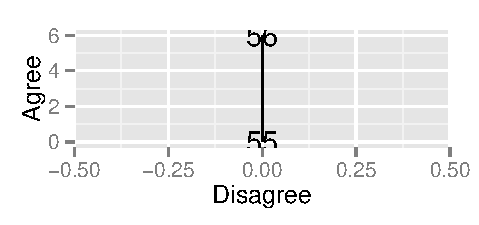
\includegraphics[width=\maxwidth]{figure/unnamed-chunk-31} 

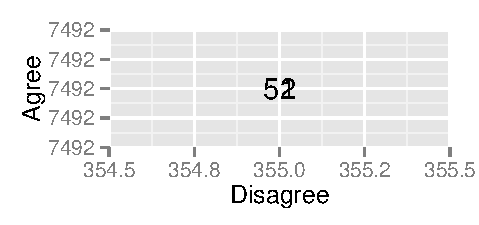
\includegraphics[width=\maxwidth]{figure/unnamed-chunk-32} 

\end{knitrout}

\caption{ROC for Gen1Housemates (left) and Gen2Siblings (right)}
\end{figure}

% latex table generated in R 3.0.0 by xtable 1.7-1 package
% Sun May 26 02:49:16 2013
\begin{table}[ht]
\centering
{\large
\begin{tabular}{lrrrrr}
  \hline
R & Implicit2004 & Implicit & Roster & Explicit & Eventual \\ 
  \hline
0 & - &   1 & 478 &  41 & 517 \\ 
  0.125 &  76 & - &  96 & - &  96 \\ 
  0.130999997258186 & - & - & - &   2 &   6 \\ 
  0.25 &  43 &  12 & - & 273 & 268 \\ 
  0.375 & 310 & - & - &  37 &  31 \\ 
  0.5 & 1877 & 2493 & - & 3598 & 3888 \\ 
  0.75 &  32 & - & - & - &  11 \\ 
  1 & - & - & - & - &  11 \\ 
  - & 2964 & 2796 & 4728 & 1351 & 474 \\ 
   \hline
\end{tabular}
}
\caption{Counts for Gen1Housemates} 
\end{table}
% latex table generated in R 3.0.0 by xtable 1.7-1 package
% Sun May 26 02:49:16 2013
\begin{table}[ht]
\centering
{\large
\begin{tabular}{lrrrrr}
  \hline
R & Implicit2004 & Implicit & Roster & Explicit & Eventual \\ 
  \hline
0 & - &   1 & 478 &  41 & 517 \\ 
  0.125 &  76 & - &  96 & - &  96 \\ 
  0.130999997258186 & - &  36 & - &   2 &   6 \\ 
  0.25 &  43 &  12 & - & 273 & 268 \\ 
  0.375 & 310 &  44 & - &  37 &  31 \\ 
  0.5 & 1877 & 2493 & - & 3598 & 3888 \\ 
  0.75 &  32 & - & - & - &  11 \\ 
  1 & - & - & - & - &  11 \\ 
  - & 2964 & 2716 & 4728 & 1351 & 474 \\ 
   \hline
\end{tabular}
}
\caption{Counts for Gen1Housemates (Previous version of links)} 
\end{table}
% latex table generated in R 3.0.0 by xtable 1.7-1 package
% Sun May 26 02:49:16 2013
\begin{table}[ht]
\centering
{\large
\begin{tabular}{lrrrr}
  \hline
R & Implicit2004 & Implicit & Explicit & Eventual \\ 
  \hline
- &   0 &   0 &   0 &   0 \\ 
   \hline
\end{tabular}
}
\caption{Counts for Gen2Siblings} 
\end{table}
% latex table generated in R 3.0.0 by xtable 1.7-1 package
% Sun May 26 02:49:16 2013
\begin{table}[ht]
\centering
{\large
\begin{tabular}{lrrrr}
  \hline
R & Implicit2004 & Implicit & Explicit & Eventual \\ 
  \hline
- &   0 &   0 &   0 &   0 \\ 
   \hline
\end{tabular}
}
\caption{Counts for Gen2Siblings (Previous version of links)} 
\end{table}



% latex table generated in R 3.0.0 by xtable 1.7-1 package
% Sun May 26 02:49:16 2013
\begin{table}[ht]
\centering
\begin{tabular}{rrrrrr}
  \hline
Count & RImplicit2004 & RImplicit & RExplicit & RRoster & Delta \\ 
  \rowcolor{goodColor}  \hline
1192 & 0.500 & 0.500 & 0.500 & - & 0 \\ 
   \rowcolor{sosoColor} 1013 & - & - & 0.500 & - & 26 \\ 
   \rowcolor{goodColor} 787 & - & 0.500 & 0.500 & - & 0 \\ 
   \rowcolor{nullColor} 391 & - & - & - & - & 3 \\ 
   \rowcolor{sosoColor} 314 & 0.500 & - & 0.500 & - & 9 \\ 
   \rowcolor{nullColor} 282 & - & - & - & 0.000 & 7 \\ 
   \rowcolor{sosoColor} 218 & - & - & 0.250 & - & 5 \\ 
  195 & 0.500 & 0.500 & - & - & 0 \\ 
   \rowcolor{sosoColor} 187 & 0.375 & - & 0.500 & - & 12 \\ 
  108 & - & 0.500 & - & - & 0 \\ 
   \rowcolor{nullColor} 60 & 0.500 & - & - & 0.000 & 2 \\ 
   \rowcolor{nullColor} 44 & 0.375 & - & - & - & 1 \\ 
  43 & 0.500 & 0.500 & - & 0.000 & 0 \\ 
  43 & - & 0.500 & - & 0.000 & 0 \\ 
   \rowcolor{nullColor} 37 & 0.125 & - & - & 0.125 & 3 \\ 
   \rowcolor{nullColor} 35 & 0.500 & - & - & - & 0 \\ 
   \rowcolor{goodColor} 34 & 0.375 & 0.500 & 0.500 & - & 0 \\ 
   \rowcolor{nullColor} 30 & - & - & - & 0.125 & 8 \\ 
   \rowcolor{sosoColor} 27 & - & - & 0.000 & - & 0 \\ 
   \rowcolor{sosoColor} 25 & - & - & 0.375 & - & 0 \\ 
   \rowcolor{sosoColor} 18 & 0.375 & - & 0.250 & - & 0 \\ 
   \rowcolor{badColor} 14 & 0.500 & 0.500 & 0.250 & - & 0 \\ 
   \rowcolor{sosoColor} 13 & 0.250 & - & 0.500 & - & 0 \\ 
  12 & 0.125 & 0.500 & - & 0.125 & 0 \\ 
   \rowcolor{sosoColor} 10 & 0.125 & - & 0.500 & - & 0 \\ 
   \rowcolor{sosoColor} 10 & 0.750 & - & 0.500 & - & 0 \\ 
   \rowcolor{nullColor} 10 & 0.375 & - & - & 0.000 & 1 \\ 
   \rowcolor{nullColor} 9 & 0.250 & - & - & 0.000 & 0 \\ 
   \rowcolor{goodColor} 9 & 0.750 & 0.500 & 0.500 & - & 0 \\ 
   \rowcolor{nullColor} 8 & 0.250 & - & - & - & 0 \\ 
   \rowcolor{badColor} 8 & - & 0.500 & 0.250 & - & 0 \\ 
   \rowcolor{goodColor} 7 & 0.250 & 0.500 & 0.500 & - & 0 \\ 
   \rowcolor{badColor} 6 & 0.500 & 0.250 & 0.500 & - & 0 \\ 
   \rowcolor{nullColor} 6 & 0.750 & - & - & - & 0 \\ 
   \rowcolor{sosoColor} 6 & - & - & 0.250 & 0.000 & 1 \\ 
   \rowcolor{sosoColor} 5 & 0.500 & - & 0.250 & - & 1 \\ 
   \rowcolor{goodColor} 4 & 0.125 & 0.500 & 0.500 & - & 0 \\ 
   \rowcolor{nullColor} 4 & 0.125 & - & - & - & 0 \\ 
  4 & 0.375 & 0.500 & - & - & 0 \\ 
   \rowcolor{sosoColor} 4 & 0.375 & - & 0.375 & - & 0 \\ 
   \rowcolor{nullColor} 4 & 0.375 & - & - & 0.125 & 0 \\ 
  4 & 0.500 & 0.500 & 0.375 & - & 0 \\ 
   \rowcolor{nullColor} 4 & 0.750 & - & - & 0.000 & 0 \\ 
  4 & - & 0.500 & - & 0.125 & 0 \\ 
   \rowcolor{sosoColor} 4 & - & - & 0.500 & 0.000 & 0 \\ 
   \rowcolor{nullColor} 3 & 0.125 & - & - & 0.000 & 0 \\ 
  3 & 0.375 & 0.500 & - & 0.000 & 0 \\ 
   \rowcolor{badColor} 3 & - & 0.250 & 0.500 & - & 0 \\ 
   \rowcolor{badColor} 3 & - & 0.500 & 0.000 & - & 0 \\ 
   \rowcolor{badColor} 2 & 0.125 & 0.500 & 0.000 & - & 0 \\ 
  2 & 0.250 & 0.500 & - & 0.000 & 0 \\ 
   \rowcolor{sosoColor} 2 & 0.250 & - & 0.250 & - & 0 \\ 
   \rowcolor{badColor} 2 & 0.500 & 0.500 & 0.000 & - & 0 \\ 
   \rowcolor{sosoColor} 2 & 0.500 & - & 0.375 & - & 0 \\ 
  2 & 0.750 & 0.500 & - & - & 0 \\ 
   \rowcolor{badColor} 2 & - & 0.500 & 0.000 & 0.000 & 0 \\ 
  2 & - & 0.500 & 0.375 & - & 0 \\ 
   \rowcolor{sosoColor} 2 & - & - & 0.000 & 0.125 & 0 \\ 
   \rowcolor{sosoColor} 1 & 0.125 & - & 0.000 & 0.125 & 0 \\ 
   \rowcolor{sosoColor} 1 & 0.125 & - & 0.000 & - & 0 \\ 
   \rowcolor{sosoColor} 1 & 0.125 & - & 0.250 & - & 0 \\ 
  1 & 0.250 & 0.500 & - & - & 0 \\ 
   \rowcolor{nullColor} 1 & 0.250 & - & - & 0.125 & 0 \\ 
   \rowcolor{goodColor} 1 & 0.375 & 0.500 & 0.500 & 0.000 & 0 \\ 
   \rowcolor{sosoColor} 1 & 0.375 & - & 0.000 & 0.000 & 0 \\ 
  1 & 0.500 & 0.250 & - & 0.125 & 0 \\ 
  1 & 0.500 & 0.250 & - & - & 0 \\ 
   \rowcolor{badColor} 1 & 0.500 & 0.500 & 0.131 & - & 0 \\ 
   \rowcolor{goodColor} 1 & 0.500 & 0.500 & 0.500 & 0.000 & 0 \\ 
  1 & 0.500 & 0.500 & - & 0.125 & 0 \\ 
  1 & 0.750 & 0.500 & - & 0.000 & 0 \\ 
  1 & - & 0.000 & - & 0.000 & 0 \\ 
  1 & - & 0.250 & - & 0.000 & 0 \\ 
   \rowcolor{goodColor} 1 & - & 0.500 & 0.500 & 0.000 & 0 \\ 
   \rowcolor{sosoColor} 1 & - & - & 0.131 & - & 0 \\ 
   \rowcolor{sosoColor} 1 & - & - & 0.250 & 0.125 & 0 \\ 
   \rowcolor{sosoColor} 1 & - & - & 0.500 & 0.125 & 0 \\ 
   \rowcolor{sosoColor} 1 & 0.125 & - & 0.500 & 0.125 & 1 \\ 
   \rowcolor{sosoColor} 0 & - & 0.375 & 0.500 & - & -24 \\ 
   \rowcolor{sosoColor} 0 & 0.375 & 0.375 & 0.500 & - & -11 \\ 
  0 & - & 0.131 & - & 0.125 & -8 \\ 
   \rowcolor{sosoColor} 0 & 0.500 & 0.375 & 0.500 & - & -7 \\ 
  0 & - & 0.131 & - & 0.000 & -7 \\ 
  0 & - & 0.131 & 0.250 & - & -4 \\ 
  0 & 0.125 & 0.131 & - & 0.125 & -3 \\ 
  0 & - & 0.131 & - & - & -3 \\ 
   \rowcolor{badColor} 0 & 0.500 & 0.131 & 0.500 & - & -2 \\ 
  0 & 0.500 & 0.131 & - & 0.000 & -2 \\ 
   \rowcolor{badColor} 0 & - & 0.131 & 0.500 & - & -2 \\ 
   \rowcolor{badColor} 0 & 0.125 & 0.131 & 0.500 & 0.125 & -1 \\ 
   \rowcolor{badColor} 0 & 0.375 & 0.131 & 0.500 & - & -1 \\ 
  0 & 0.375 & 0.131 & - & 0.000 & -1 \\ 
  0 & 0.375 & 0.131 & - & - & -1 \\ 
   \rowcolor{sosoColor} 0 & 0.500 & 0.375 & 0.250 & - & -1 \\ 
  0 & - & 0.131 & 0.250 & 0.000 & -1 \\ 
   \rowcolor{sosoColor} 0 & - & 0.375 & 0.250 & - & -1 \\ 
   \hline
\end{tabular}
\caption{Counts for Gen1Housemates} 
\end{table}



\end{document}
